\chapter{Research Method}


%===================================================================================================%
\section{Introduction}
%===================================================================================================%

After exploring the academic body of knowledge in chapter \ref{chp:background}, 


%===================================================================================================%
\section{Method Evaluation}
%=======================================================%

There are several competing methodological approaches to assess the aptness of technologies in the domain of information systems. In the following section four of these are introduced, discussed and evaluated for further use:

\begin{enumerate}
    
    %-------------------------------------%
    \item \textbf{Task-Technology-Fit}\\
    %-------------------------------------%
    \begin{figure}[ht]
        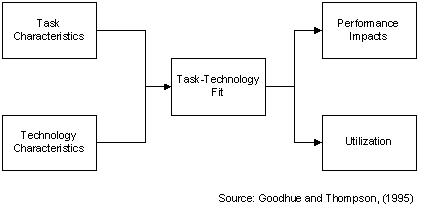
\includegraphics[width=0.7\linewidth]{images/methodology/ttf.jpg}\centering
        \caption
        [Task-Technology-Fit Model]
        {Task-Technology-Fit Model \cite{Goodhue1995Task-TechnologyPerformance}}
    \end{figure}
    
    One of the oldest holistic models for assessing the fit of a given technology is called the "Task-Technology-Fit" (TTF) model. It originates in 1995 and is based on theories of user attitudes, beliefs and behaviors. It implies that a better fit of a technology for a task will result in increased utilization and will have a positive performance impact. Goodhue and Thompson developed a measure that consists of the eight factors:
    \begin{enumerate}
        \item[\textbf{1}] Quality
        \item[\textbf{2}] Locatability
        \item[\textbf{3}] Authorization
        \item[\textbf{4}] Compatibility
        \item[\textbf{5}] Ease of Use/Training
        \item[\textbf{6}] Production Timeliness
        \item[\textbf{7}] Systems Reliability
        \item[\textbf{8}] Relationship with Users
    \end{enumerate}
    It is apparent that these eight factors are focused on the user of the technology and rely on subjective user-perception. Although Goodhue and Thompson developed their methodology for the individual level of analysis, Zigurs and Buckland refined it for application on group level.\autocite{Zigurs1998AEffectiveness} As mentioned before, this basic TTF model heavily relies on the subjective perception of the user and therefore often operates with surveys or interviews. Since TTF is a very generalistic and holostic approach, it was applied on various domains of information systems and has been combined or used with other related models with great success.\\ 
    However, it is very uncommon to use the TTF in its original, unaltered form but rather modify it to suit the purpose of the particular study since different fields of study require different validation methods. For the technical evaluation of serverless architectures in the context of IoT Event-Stream-Processing the TTF perspective of defining \textit{Task Characteristics} and \textit{Technology Characteristics} to assess the fit and therefore the \textit{Performance Impacts} and \textit{Utilization} but the suggested validation methods (i.e., survey or interview) are not applicable for this study. It is therefore necessary to look at different models and define a research methodology that is fitting for the study at hand. 
    
     %-------------------------------------%
    \item \textbf{Fit-Viability Model}\\
    %-------------------------------------%
    \begin{figure}[ht]
        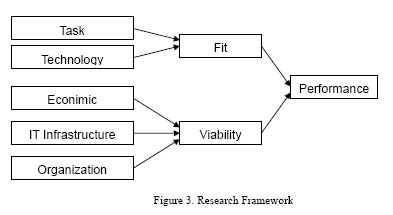
\includegraphics[width=0.7\linewidth]{images/methodology/fvm.jpg}\centering
        \caption
        [Fit-Viability-Model]
        {Fit-Viability-Model \cite{Liang2007AdoptionModel}}
    \end{figure}
    The "Fit-Viability Model" (FVM) for evaluating organizational adoption of technologies was originally proposed by Tjan in 2001 and refined by Liang in 2007. As an extension of the Task-Technology-Fit model it adopts the technology's fit but also introduces the "viability" dimension. Similarly to the approach outline in the last paragraph, FVM assesses the fit be evaluating how well the studied technology fits for the given task in order to gain insights on how well it impacts the performance and utilization. The added dimension of viability is very interesting and important for this study since it includes the economic perspective on the solution and also enables the researcher to focus on the realistic implementation and use of the technology. Similarly to TTF, it is rather vague in recommending specific validation methods and needs to be modified to fit the study. 
    
    %-------------------------------------%
    \item \textbf{Prototyping}\\
    %-------------------------------------%
    "Prototyping" refers to the practice of building functioning versions of a system in order to observe its behaviour and derive conclusions on how the productive version would behave.\autocite{Budde1992Prototyping} Since it is a common approach for business and hobbyists alike, a concise and generally accepted definition is hard to find because the understanding can differ vastly depending on the person or organization using it. For research purpose, this paper focuses on the two most important academic sources on the topic: Budde (1992) and Nielsen (1993).\\
    Nielsen defines two different types of prototypes:
    
    \begin{figure}[ht]
        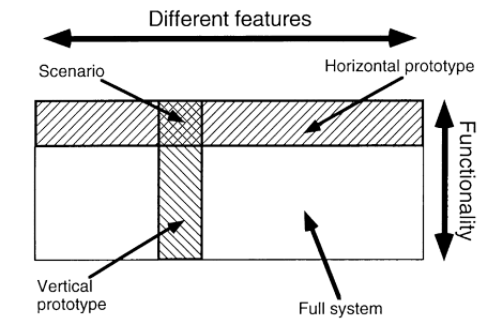
\includegraphics[width=0.7\linewidth]{images/methodology/nielsenProto.PNG}\centering
        \caption
        [The two dimensions of prototyping]
        {The two dimensions of prototyping \cite{Nielsen1993UsabilityEngineering}}
    \end{figure}
    
    \begin{enumerate}
        \item \textbf{Horizontal Prototype}\\
            By reducing the level of functionality, the result of horizontal prototyping is \blockquote{a simulation of the interface where no real work can be performed. [...] This would mean that users should be able to execute all navigation and search commands but without retrieving any real information as a result of these commands}.\autocite{Nielsen1993UsabilityEngineering} The goal is to test the entire user interface without needing to develop the underlying systems. The main advantage of horizontal prototyping is that it provides a rapid feedback-loop between researcher and user by reducing the development time but still delivering a fully functional prototype. In addition, a quick, cost-effective confirmation of the requirements and system scope can be done and first estimates of development time, cost and effort conducted. Moreover, it is an excellent way to showcase the running system to gain a business advantage.\autocite{Nielsen1993UsabilityEngineering}
        \item \textbf{Vertical Prototype}\\
            A vertical prototype is a system that features in-depth functionality but only for a few selected features. Hence, it only provides sufficient test data for a limited part of the system, but it will be tested thoroughly under near real-life conditions. For instance, a vertical prototype of a concert ticket system could feature a fully functional API and processing unit but mocks the database in order to assess only the API and processing unit. 
    \end{enumerate}
    
    Prototyping can be the used to solve various problems and depending on the goal the overall approach can differ vastly. Floyd\autocite{Floyd1984APrototyping} distinguishes between three particular styles of prototyping relating to different goals:
    
    \begin{enumerate}
        \item \textbf{Exploratory Prototyping}\\
            When the problem is unclear, exploratory prototyping is an apt approach for testing initial ideas in order to gain perspective on user and management requirements. Usually, the main focus is to examine a broad variety of design options and to explore these options without premature assumptions or restrictions. As a result, the developer can "play" with various design choices and gain insight into the users' perception of the application. 
        \item \textbf{Experimental Prototyping}\\
            This form of prototyping is closely related to \textit{exploratory prototyping} but focuses on the technical implementation of the development goal. By designing reference systems within the defined problem's scope, 
    \end{enumerate}
    
    Since this study aims to answer the question whether and under which circumstances serverless architectures are a good fit for IoT Event-Stream-Processing, an experimental, vertical prototype is better suited as a method of validation. 
    
    %-------------------------------------%
    \item \textbf{Requirements Engineering}\\
    %-------------------------------------%
    
    \blockquote{\guillemotleft \ Requirements engineering is the branch of software
    engineering concerned with the real-world goals for,
    functions of, and constraints on software systems. It
    is also concerned with the relationship of these
    factors to precise specifications of software behavior,
    and to their evolution over time and across software
    families." \guillemotright\autocite{Zave1997ClassificationEngineering}}
    
    This definition is very appealing for a number of reasons. To begin with, it emphasizes the focus on "real-world goals" that have to addressed in order to create value. These goals define \textit{why} the system should be built and \textit{what} the system's purpose is. In addition, it mentions "precise specification" which provide the the basis for requirements that shape how the software will behave. \textit{Requirements Engineering} is therefore the method of defining and documenting requirements for a software. There is no specific, generally accepted toolset of best practices and methods but rather a common understanding what requirements engineering should achieve: 
    \begin{itemize}
        \item Identification of Requirements\\
            Understand the features and functionality the task's environment demands
        \item System Modeling (see \textit{Prototyping})\\
            Design a reference system 
        \item Requirements Specification\\
            Specify the identified requirements further
        \item Requirements Validation\\
            Validate the identified and specified requirements
    \end{itemize}\autocite{Budde1992Prototyping}\autocite{Sommerville1999RequirementsGuide}\autocite{Sommerville2010SoftwareEngineering}
    
    
    
\end{enumerate}








%===================================================================================================%
\section{Prototyping}
%=======================================================%

managed container: IBM IoTP\\
serverless: AWS Kinesis+Firehose+Lambda

%***************%
\section{Requirement Engineering and Operationalization}\label{sec:operationalization}
%***************%

%***************%
\subsection{Viability Assessment}
%***************%

\begin{figure}[ht]
    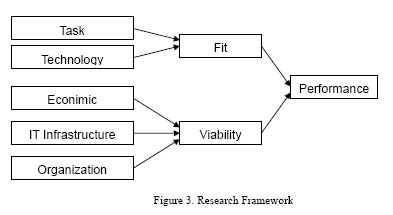
\includegraphics[width=0.7\linewidth]{images/methodology/fvm.jpg}\centering
    \caption
    [Fit-Viability-Model]
    {Fit-Viability-Model \cite{Liang2007AdoptionModel}}
\end{figure}

\subsubsection{Hypothesis: Serverless}

\textbf{Properties that are rather positive:}
\begin{enumerate}\label{lst:viabPro}
    \item provisioning
    \item security
    \item ease of deployment
    \item documentation
    \item metrics
    \item rollback
\end{enumerate}

\textbf{Aspects that can neutral or negative effect:}
\begin{enumerate}\label{lst:viabCon}
    \item tooling (especially API creation)
    \item docs
    \item vendor lock-in (serverless = "servicefull")
\end{enumerate}

%***************%
\subsection{Suitability Assessment}
%***************%

\subsubsection{Hypothesis: Serverless}

\textbf{Properties that are rather positive:}
\begin{enumerate}\label{lst:suitPro}
    \item scalability
    \item microbilling
    \item "limitless" auto-scaling. "you don't think about scaling"
    \item loosely coupled
    \item event-driven
\end{enumerate}

\textbf{Properties that can neutral or negative effect:}
\begin{enumerate}\label{lst:suitCon}
    \item stateless 
    \item limited execution time
    \item startup latency ("coldstart")
    \item 
    \item execution duration (long running jobs)
\end{enumerate}


\begin{figure}[ht]
    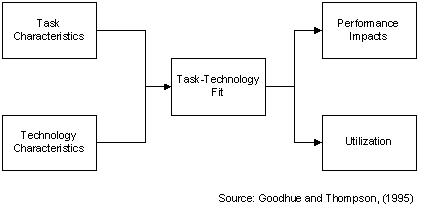
\includegraphics[width=0.7\linewidth]{images/methodology/ttf.jpg}\centering
    \caption
    [Task-Technology-Fit Model]
    {Task-Technology-Fit Model \cite{Goodhue1995Task-TechnologyPerformance}}
\end{figure}


%===================================================================================================%
\section{Summary}
%===================================================================================================%